%----------------------------------------------%
%            Package Indispensables            %
%----------------------------------------------% 
\documentclass[a4paper]{article}
\usepackage[utf8x]{inputenc}
\usepackage[T1]{fontenc}
%\usepackage[french]{babel} 
\usepackage[francais,bloc,ensemble,nowatermark,outsidebox]{automultiplechoice} % Pour utiliser AMC
\usepackage{multicol}% pour pouvoir mettre les réponses sur plusieurs colonnes

%----------------------------------------------%
%          Options de mise en page             %
%----------------------------------------------%
% Espacemements - marges
\geometry{includehead,includefoot,left=60pt,right=60pt,top=40pt,bottom=50pt,headsep=30pt,footskip=20pt} 

% Espacemements - paragraphes
\setlength{\parskip}{20pt} % espace entre 2 paragraphes
\setlength\parindent{0pt}  % indentation en début de paragraphe

% Espacemements - questionnaire
\AMCinterIrep=3pt    % espace entre chaques réponses
\AMCinterBquest=0pt  % espace entre chaques questions (+ espace entre paragraphes)
\setlength{\multicolsep}{5pt} % espace entre questions et réponses

% Espacemements - formulaire
\AMCformHSpace=3pt  % espace entre chaques réponses 
\AMCformVSpace=-7pt  % espace entre chaques questions (+ espace entre paragraphes)

% Espacemements - figures
\setlength{\intextsep}{20pt plus 2pt minus 2pt}    % espace sup et inf quand dans le texte 
\setlength{\textfloatsep}{20pt plus 2pt minus 2pt} % espace sup et inf quand hors du texte
\setlength{\abovecaptionskip}{5pt} % espace au dessus d'une légende
\setlength{\belowcaptionskip}{0pt} % espace au dessous d'une légende

% Mise en forme des titres de section
\usepackage{titlesec} 
\renewcommand\thesection{\Roman{section}}        % Police section
\renewcommand\thesubsection{\arabic{subsection}} % Police sous-section
\titleformat{\section}[block]{\Large\scshape}{\thesection.}{1em}{} % Style de la section
\titleformat{\subsection}[block]{\normalfont\bfseries}{\thesection.\thesubsection.}{1em}{} % Style de la sous-section

\AMCboxStyle{shape=none} % style des cases dans le questionaire
\def\AMCchoiceLabel#1{\Alph{#1})} % numéro des cases dans le questionaire
% pour le style et numéro des case dans le formulaire de réponses, voir tous en bas


%----------------------------------------------%
%             Packages Optionels               %
%----------------------------------------------% 
\usepackage{enumitem} % Customized lists
\setlist[itemize]{noitemsep} % Make itemize lists more compact
\usepackage[font=footnotesize,labelfont=bf,textfont=it,justification=justified,singlelinecheck=false,position=below]{caption}
\usepackage{amsmath,amsfonts,amssymb}
\usepackage{mathtools}
\usepackage{tabularx}
\usepackage{graphicx} % gère les figures 
\usepackage{pdfpages} % on peut inclure des pages pdf
\usepackage{etoolbox} 
\usepackage{xspace} % xspace so that spaces after commands are handled correctly
\raggedbottom % tout l'extra spacing se fait en bas de page
\pdfpageattr{/Group << /S /Transparency /I true /CS /DeviceRGB>>} % enève la transparence pour qu'il n'y ai pas de problème d'affichage ou d'impression (texte plus gras si image avec fond transparent sur la page)
\usepackage{chngcntr}
\usepackage{blindtext}

%\AMCsetFoot{copie \AMCStudentNumber page \thepage}
% le code en haut de la page = copie/page/page totale


%----------------------------------------------%
%                   Barème                     %
%----------------------------------------------% 
\baremeDefautS{b=1,m=0,e=0,v=0} % barème questions simples
\baremeDefautM{b=1,m=-1,e=0,v=0} % barème questions multiples
% b = points pour bonne rép
% m = points pour mauvaise rép
% e = note affectée si plusieurs cases cochées pour une question simple
% v = La note affectée en cas de non-réponse (aucune case n’est cochée)
% mz = ”maximum ou zéro” : doit cocher toutes et uniquement les bonnes réponses pour avoir la note mz sinon, elle sera nulle.


%----------------------------------------------%
%                  Document                    %
%----------------------------------------------% 
\begin{document}

\AMCrandomseed{10} % choisir entre 1 et 4194303 >> définit le mélange des questions

% Style des questions
\def\AMCbeginQuestion#1#2{\par\noindent{Question #1} #2\vspace{3pt} \hrule \vspace{8pt}}
\def\multiSymbole{} % symbole signifiant qu'il y a plusieurs réponses possibles
% Style formulaire
\def\AMCformQuestion#1{Question #1 :}
\def\AMCotextReserved{\emph{Réservé à l'enseignant}} % texte pour les questions ouvertes

\exemplaire{59}{ % nombre de copies différentes

%----------------------------------------------%
%                   En-tête                    %
%----------------------------------------------%
\begin{center}
  {\huge Projet Conception de Convertisseurs} \\
  \vspace{10pt}
  Semestre 8 - Département 3EA\\ 
  Enseignants : M. Cousineau - G. Fontès - A. Jaafar - H. Schneider - N. Roux - S. Suarez\\
  Date: 15 décembre 2025
\end{center}

\begin{center}\fbox{\fbox{\parbox{0.95\textwidth}{
\begin{itemize}[label=\textbullet,font=\footnotesize, leftmargin=15pt]
\item En haut à droite de vos feuille : verifiez que le premier des trois numéros soit toujours le même.
\item Les réponses aux questions sont à donner EXCLUSIVEMENT sur la feuille de réponses.
\item Les cases doivent être entièrement noircies avec un stylo noir ou bleu.
\item En cas d'erreur, appliquer du blanc (mais ne surtout pas redessiner la case). 
\end{itemize}}}}
\end{center}

%----------------------------------------------%
%                 Questions                    %
%----------------------------------------------%

\begin{question}{Question1}
Dans un hacheur dévolteur à tension d'entrée constante, pour augmenter la tension moyenne de sortie, on peut :
	\begin{multicols}{2}
	\begin{reponses}
		\bonne{augmenter le rapport cyclique}
		\mauvaise{augmenter la fréquence de découpage}
        \mauvaise{augmenter la fréquence de coupure du filtre de sortie}
	\end{reponses}
	\end{multicols}
\end{question}

\begin{question}{Question2}
Pour implémenter une commande analogique d'un hacheur dévolteur, on comparera une porteuse triangulaire comprise entre 0 et 10 V et une modulante constante.
Pour fixer un rapport cyclique de 0,6, je dois fixer la modulante constante à :
	\begin{multicols}{2}
	\begin{reponses}
        \bonne{6 V}
        \mauvaise{4 V}
        \mauvaise{0,6 V}
        \mauvaise{0,4 V}
	\end{reponses}
	\end{multicols}
\end{question}

\begin{question}{Question3}
On considère une topologie de hacheur dévolteur avec une tension d'entrée de 250 V, une fréquence de découpage de 2,5 kHz et un rapport cyclique de 0,4.
Quelle sera la tension moyenne de sortie ?
	\begin{multicols}{2}
	\begin{reponses}
		\bonne{100 V}
		\mauvaise{10 V}
		\mauvaise{1 000 V}
		\mauvaise{40 V}
	\end{reponses}
	\end{multicols}
\end{question}

\begin{question}{Question4}
L'énergie perdue par commutation (amorçage et blocage) dans un IGBT au point  600V-40A est de 6 mJ. Quelles seront les pertes par commutation à 5 kHz au point 300V-40A ?
	\begin{multicols}{2}
	\begin{reponses}
		\bonne{15 W}
		\mauvaise{30 W}
		\mauvaise{60 W}
		\mauvaise{150 W}
	\end{reponses}
	\end{multicols}
\end{question}


\begin{question}{Question5}
La tension $V_{CE_{on}}$ de l'IGBT à l'état passant est de 2 V sous 40 A. Quelles seront les pertes en conduction pour un rapport cyclique de 0.25 ?
	\begin{multicols}{2}
	\begin{reponses}
		\bonne{20 W}
		\mauvaise{20 J}
		\mauvaise{80 W}
		\mauvaise{80 J}
	\end{reponses}
	\end{multicols}
\end{question}

\begin{question}{Question6}
Un module IGBT est monté sur un radiateur de résistance thermique 0,2 K/W. Au point nominal les pertes totales dans le module sont de 100 W. Quelle sera la différence de température entre l'air ambiant et la semelle du composant ?
	\begin{multicols}{2}
	\begin{reponses}
		\bonne{20 °C}
		\mauvaise{20 K/W}
		\mauvaise{0,002 °C}
        \mauvaise{0,002 K/W}
	\end{reponses}
	\end{multicols}
\end{question}

\begin{question}{Question7}
Un onduleur MLI monophasé - avec \emph{modulation 3 niveaux (modulation unipolaire)} - dont la fréquence de découpage des interrupteurs semiconducteurs vaut 10 kHz comporte un filtre de sortie du $2^{\Grave{e}me}$ ordre dont la fréquence propre est égale à 2 kHz. Les premiers harmoniques dus aux découpage seront atténués d'un rapport :
	\begin{multicols}{2}
	\begin{reponses}
		\bonne{100}
		\mauvaise{25}
		\mauvaise{5}
		\mauvaise{10}
	\end{reponses}
	\end{multicols}
\end{question}





\begin{questionmult}{Question8}
La figure ci-après présente les formes d'ondes en simulation d'un onduleur monophasé : sur le graphe du haut tension de sortie et courant de sortie, sur le graphe du bas tension interrupteur $K_3$ et courant interrupteur $K_3$.
Que peut-on affirmer d'après ces formes d'ondes ?
	\begin{multicols}{2}
	\begin{reponses}
		\bonne{la charge est de nature inductive}
        	\bonne{les interrupteurs doivent être bidirectionnels en courant}
		\bonne{les interrupteurs sont à amorçage spontanés}
        	\bonne{les interrupteurs sont à blocage commandé}
		\mauvaise{les interrupteurs doivent être bidirectionnels en tension}
		\mauvaise{les interrupteurs sont à blocage spontané}
	\end{reponses}
	\end{multicols}
\end{questionmult}

\begin{figure}[h!]
	\centering
	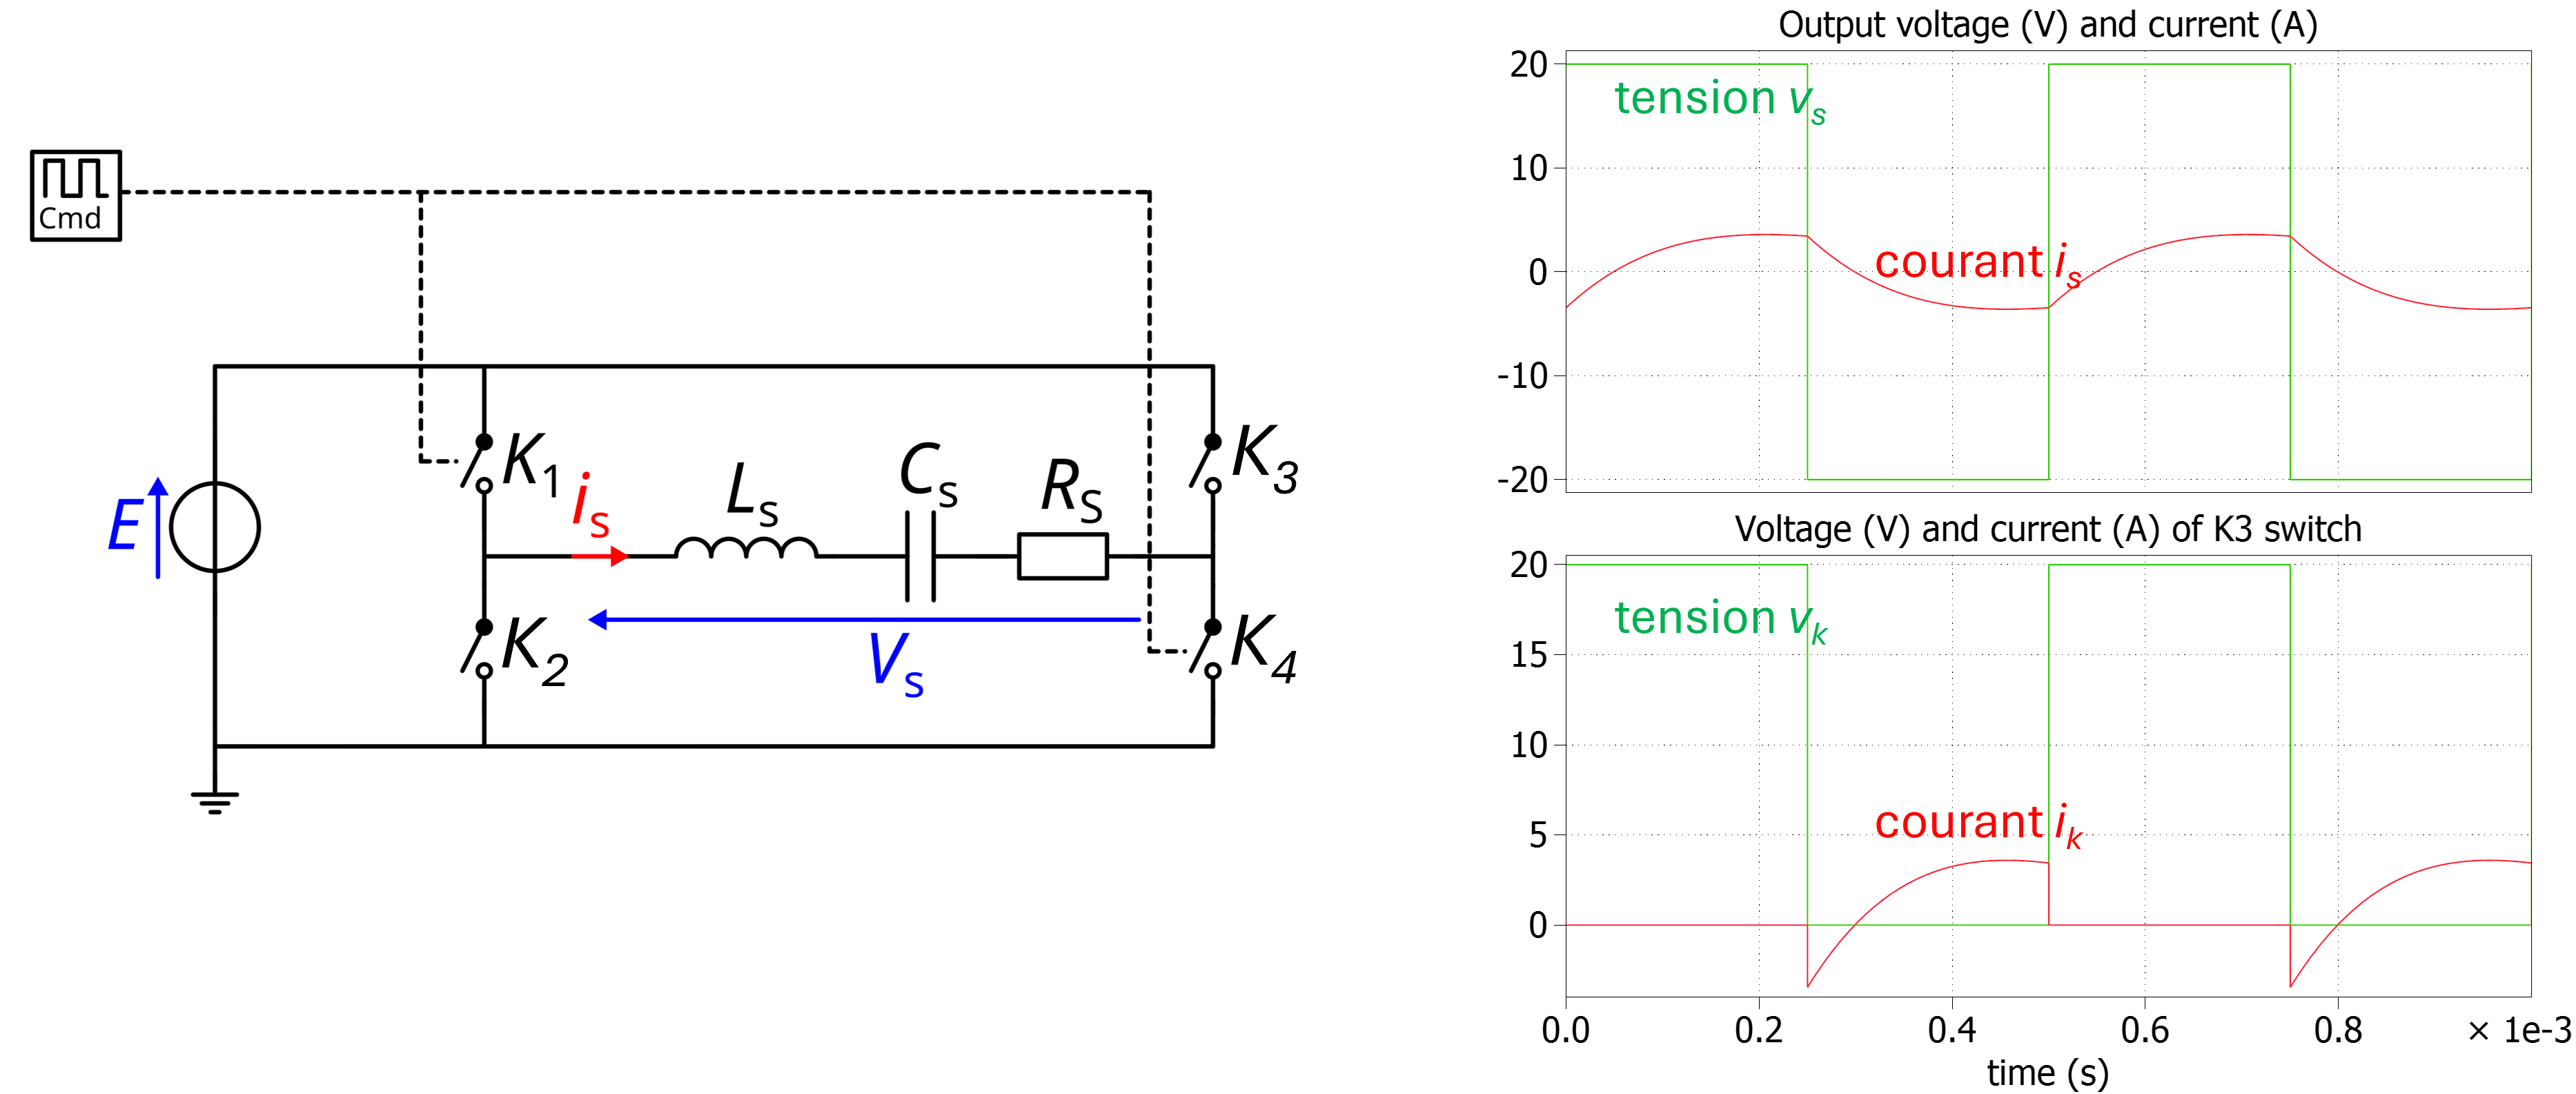
\includegraphics[width=0.9\textwidth]{Figures/vs_is_vk_ik_dephasage_ar.png}
\end{figure}





\begin{questionmult}{Question9}
La figure ci-après présente les formes d'ondes expérimentales d'un onduleur monophasé : en bleu la tension de sortie, en rose le courant.
Que peut-on affirmer d'après ces formes d'ondes ?
        \begin{multicols}{2}
        \begin{reponses}
            \bonne{la charge est de nature capacitive}
            \bonne{les interrupteurs doivent être bidirectionnels en courant}
            \bonne{les interrupteurs sont à blocage spontané}
            \mauvaise{les interrupteurs sont à amorçage spontanés}
            \mauvaise{les interrupteurs doivent être bidirectionnels en tension}
            \mauvaise{les interrupteurs sont à blocage commandé}
        \end{reponses}
        \end{multicols}
    \end{questionmult}
    
\begin{figure}[h!]
	\centering
	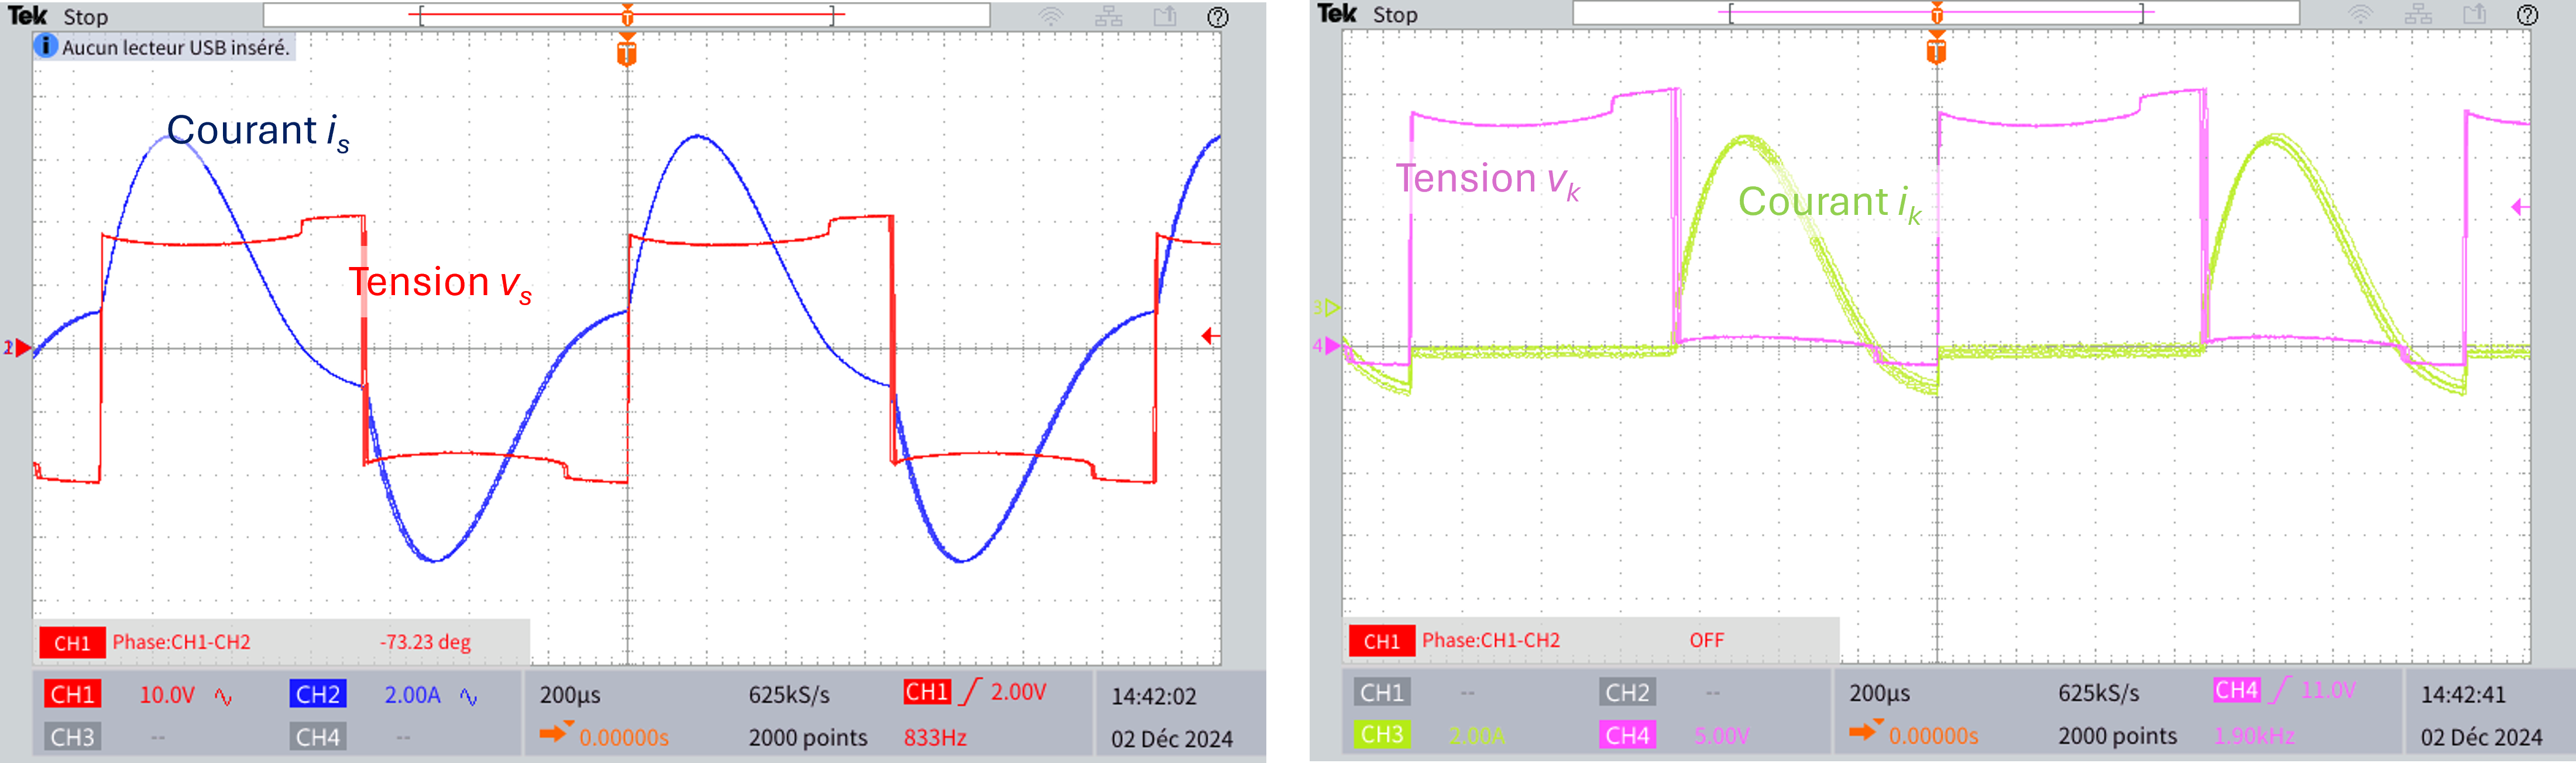
\includegraphics[width=0.9\textwidth]{Figures/vs_is_vk_ik_dephasage_av.png}
\end{figure}

\begin{questionmult}{Question10}
    Nous avons deux hacheurs dévolteurs qui alimentent une charge en différentiel. Pour les deux hacheurs, les porteuses sont triangulaires comprises entre 0 V et 10 V. Parmi les propositions suivantes de combinaisons de modulantes des deux hacheurs, laquelle permet d'obtenir une tension alternative aux bornes de la charge ?
        \begin{multicols}{2}
        \begin{reponses}
            \bonne{Bras 1 : modulante sinus à valeur moyenne de 5 V ; Bras 2 : modulante constante de 5 V}
            \mauvaise{Bras 1 : modulante sinus à valeur moyenne nulle ; Bras 2 : modulante constante de 0 V}
            \mauvaise{Bras 1 : modulante sinus à valeur moyenne de 5 V ; Bras 2 : modulante constante de 0 V}
            \mauvaise{Bras 1 : modulante sinus à valeur moyenne de 5 V ; Bras 2 : modulante sinus à valeur moyenne de 5 V}
        \end{reponses}
        \end{multicols}
    \end{questionmult}

%----------------------------------------------%
%          Formulaire de réponses             %
%----------------------------------------------%
\AMCcleardoublepage
\AMCdebutFormulaire

\begin{center}
  {\huge Feuille de réponses} \\
  \vspace{10pt}
Les réponses aux questions sont à donner EXCLUSIVEMENT sur cette feuille\\
\end{center}

\hfill\champnom{
\fbox{\parbox{0.4\textwidth}{
\vspace*{15pt}
Nom :\dotfill 
\vspace*{10pt}
}}}

\AMCboxStyle{shape=square} % style des cases dans le formulaire
\def\AMCchoiceLabel##1{\Alph{##1}} % numéro des cases dans le questionaire
\formulaire    

\AMCcleardoublepage
}

\end{document}
